\documentclass[11pt,a4paper]{article}
\usepackage[utf8]{inputenc}
\usepackage[margin=2.5cm]{geometry}
\usepackage{amsmath,amssymb}
\usepackage{graphicx}
\usepackage{booktabs}
\usepackage{siunitx}
\usepackage{hyperref}
\usepackage{caption}
\usepackage{multirow}
\usepackage[section]{placeins}

\title{Monte Carlo Simulation of the Generalized Solid-on-Solid Model}
\author{}
\date{}

\begin{document}
\maketitle

%% ============================================================
\section{Model}
%% ============================================================

We study the generalized Solid-on-Solid (SOS) model on a two-dimensional
$L\times L$ square lattice with periodic boundary conditions.
The height field $h_i\in\mathbb{R}$ is defined on each lattice site $i$,
and the Hamiltonian reads
\begin{equation}
  \mathcal{H} = K \sum_{\langle i,j\rangle} |h_i - h_j|^{\sigma},
\end{equation}
where the sum runs over all nearest-neighbor pairs, $K>0$ is the coupling
constant, and $\sigma>0$ controls the stiffness of the interface.
The purpose of the simulation is to test how the microscopic exponent
$\sigma$ affects local statistics while leaving the long-wavelength behavior
of the interface unchanged. To remove the trivial translational zero mode,
we enforce $\sum_i h_i = 0$ after every sweep; this shifts all heights by the
same constant and therefore does not affect any observables built from height
differences or nonzero Fourier modes.

%% ============================================================
\section{Simulation Algorithm}
%% ============================================================

We employ a hybrid Monte Carlo scheme combining local and nonlocal updates.
The local Metropolis move samples the microscopic distribution directly,
while the cluster move accelerates equilibration of long-wavelength modes.

\paragraph{Metropolis single-site update.}
In each sweep, $N=L^2$ sites are visited at random.
A trial move $h_i \to h_i + \delta$ with $\delta$ drawn uniformly from
$[-1,1]$ is accepted with probability $\min(1, e^{-\Delta E})$.
After each sweep the zero mode is subtracted.

\paragraph{Swendsen--Wang cluster update.}
Every 5 Metropolis sweeps, a cluster update is performed.
A random reference height $h_{\mathrm{ref}}$ is chosen, and each site is
assigned a binary spin $s_i = \mathrm{sign}(h_i - h_{\mathrm{ref}})$.
Neighboring sites with the same spin are bonded with probability
\begin{equation}
  p_{ij} = 1 - \exp\!\bigl(-\Delta E_{ij}\bigr),
  \quad
  \Delta E_{ij} = K\,|2h_{\mathrm{ref}} - h_i - h_j|^{\sigma}
                - K\,|h_i - h_j|^{\sigma},
\end{equation}
when $\Delta E_{ij}>0$; otherwise no bond is formed.
Connected clusters are identified via a union-find data structure,
and each cluster is independently flipped ($h_i \to 2h_{\mathrm{ref}} - h_i$)
with probability $1/2$.

%% ============================================================
\section{Measured Observables}
%% ============================================================

Two observables are measured after each sweep during the measurement phase:

\begin{enumerate}
\item \textbf{Surface roughness} (mean-square height fluctuation):
\begin{equation}
  M^2 = \frac{1}{N}\sum_{i=1}^{N} h_i^2.
\end{equation}

\item \textbf{Structure factor at minimum wavevector} $k_{\min}=2\pi/L$:
\begin{equation}
  \chi_{k_{\min}} = |\hat{h}_{k_{\min}}|^2 / N,
\end{equation}
where $\hat{h}_k = \sum_i h_i\, e^{i k x_i}$.
\end{enumerate}

Statistical errors are estimated via a blocking analysis with block size 100.

%% ============================================================
\section{Simulation Parameters}
%% ============================================================

\begin{table}[h]
\centering
\caption{Simulation parameters.}
\begin{tabular}{ll}
\toprule
Parameter & Value \\
\midrule
System sizes $L$        & 4, 8, 16, 32, 64, 128, 256, 512; 1024 for CG only \\
Interaction exponent $\sigma$ & 0.5, 1.0, 2.0, 4.0 \\
Coupling constant $K$   & 1.0 \\
Temperature $T=1/K$     & 1.0 \\
Thermalization sweeps    & 10\,000 \\
Measurement sweeps       & 100\,000 \\
Cluster update frequency & every 5 Metropolis sweeps \\
Block size (error est.)  & 100 \\
\bottomrule
\end{tabular}
\end{table}

Unless otherwise stated, all parameter choices are shared across the finite-size
scaling and coarse-graining analyses; the only additional system size is
$L=1024$, which is used exclusively for the real-space coarse-graining study.

%% ============================================================
\section{Results}
%% ============================================================

\subsection{Finite-Size Scaling Plots}

\begin{figure}[htbp]
\centering
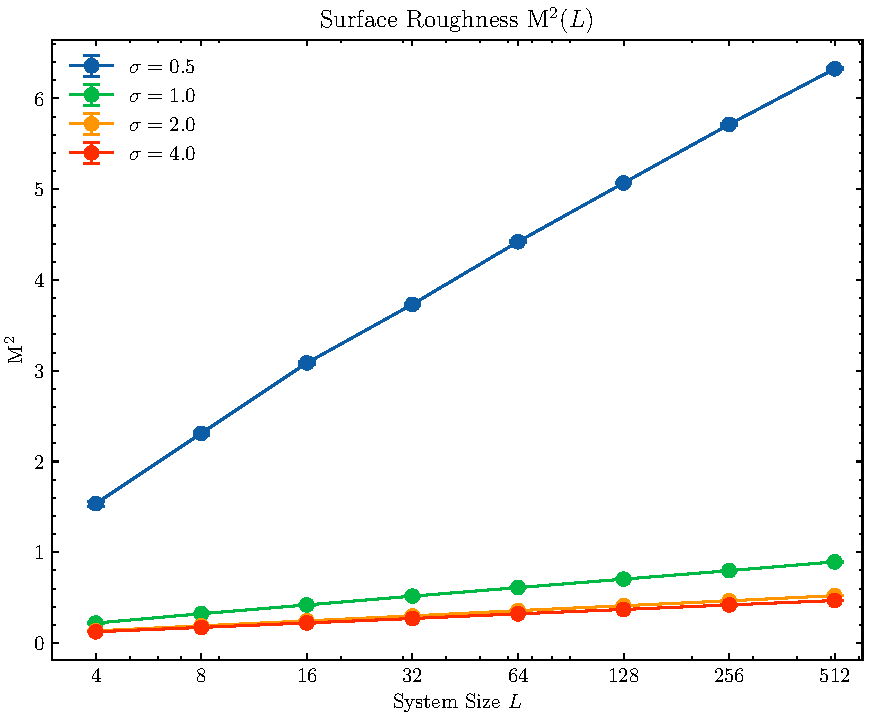
\includegraphics[width=0.75\textwidth]{../figures/W2_scaling.pdf}
\caption{Surface roughness $M^2$ as a function of system size $L$ for
different values of $\sigma$. The logarithmic growth $M^2 \sim a\ln L + b$
is characteristic of a rough phase.}
\label{fig:W2}
\end{figure}

\begin{figure}[htbp]
\centering
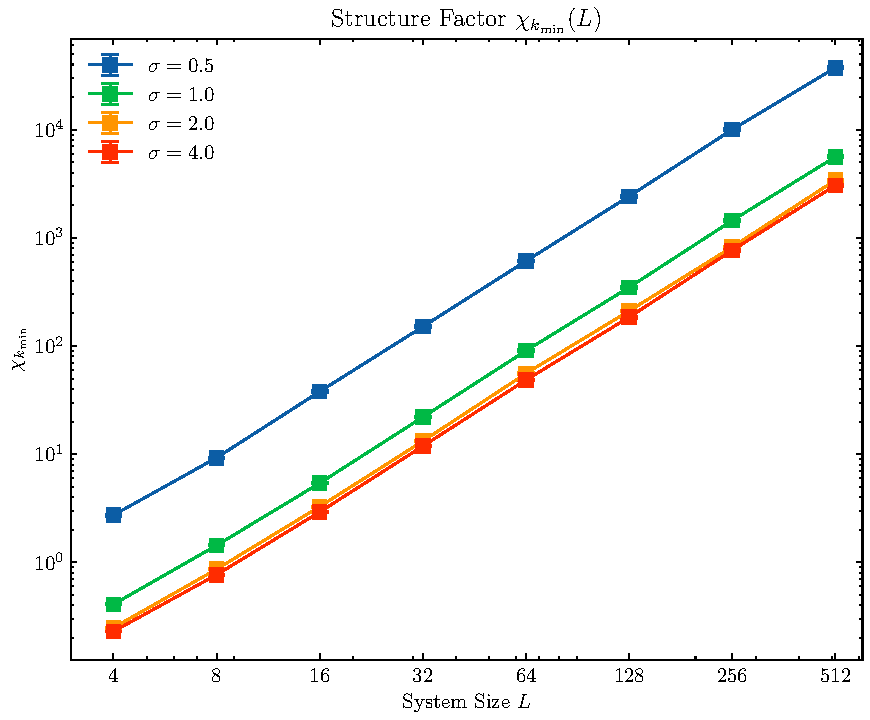
\includegraphics[width=0.75\textwidth]{../figures/chi_scaling.pdf}
\caption{Structure factor $\chi_{k_{\min}}$ vs.\ system size $L$ on a
log--log scale. The power-law scaling $\chi \sim L^{\alpha}$ with
$\alpha\approx 2$ is expected from equipartition.}
\label{fig:chi}
\end{figure}

\clearpage
\subsection{Fitting Results}

To assess finite-size corrections, we perform fits starting from
progressively larger $L_{\min}$ up to $L=512$.
The roughness is fitted to $M^2 = a\ln L + b$ (weighted linear regression
in $\ln L$), while $\chi$ is fitted to a power law
$\sim A\, L^{\alpha}$ (weighted linear regression in log--log space).
The reduced chi-squared $\chi^2_\nu$ quantifies the goodness of fit;
$\chi^2_\nu \approx 1$ indicates a good fit, while $\chi^2_\nu \gg 1$
signals significant finite-size corrections.

Across all four values of $\sigma$, the same pattern emerges. The roughness
$M^2$ is well described by $a\ln L+b$, with the prefactor $a$ decreasing
strongly as $\sigma$ increases. By contrast, $\chi_{k_{\min}}$ converges to
the universal exponent $\alpha=2$, indicating that the long-wavelength sector
is insensitive to the microscopic interaction.
The smallest lattice, $L=4$, produces the largest $\chi^2_\nu$ values and
should be regarded as pre-asymptotic data, whereas fits with $L_{\min}\ge 8$
or 16 are already close to the scaling regime.

%% ---------- sigma = 0.5 ----------
\begin{table}[htbp]
\centering
\caption{Fit results for $\sigma=0.5$.}
\label{tab:fit05}
\small
\begin{tabular}{@{}llcS[table-format=1.5]S[table-format=1.5]S[table-format=1.5]S[table-format=2.5]@{}}
\toprule
Observable & $L_{\min}$ & $N_{\mathrm{pts}}$ & {Slope/$\alpha$} & {Error} & {$R^2$} & {$\chi^2_\nu$} \\
\midrule
\multirow{5}{*}{$M^2 \sim a\ln L + b$}
 & 4  & 8 & 0.95783 & 0.00307 & 0.99753 & 20.90001 \\
 & 8  & 7 & 0.94821 & 0.00331 & 0.99883 & 12.89293 \\
 & 16 & 6 & 0.93695 & 0.00373 & 0.99972 &  5.28939 \\
 & 32 & 5 & 0.93327 & 0.00445 & 0.99957 &  6.28613 \\
 & 64 & 4 & 0.91748 & 0.00603 & 0.99984 &  1.91735 \\
\midrule
\multirow{5}{*}{$\chi \sim L^{\alpha}$}
 & 4  & 8 & 1.98963 & 0.00400 & 0.99978 &  7.56304 \\
 & 8  & 7 & 2.00167 & 0.00447 & 0.99995 &  1.85506 \\
 & 16 & 6 & 1.99689 & 0.00570 & 0.99993 &  1.85807 \\
 & 32 & 5 & 1.99457 & 0.00794 & 0.99987 &  2.41917 \\
 & 64 & 4 & 1.98625 & 0.01148 & 0.99978 &  3.12485 \\
\bottomrule
\end{tabular}
\end{table}

%% ---------- sigma = 1.0 ----------
\begin{table}[htbp]
\centering
\caption{Fit results for $\sigma=1.0$.}
\label{tab:fit10}
\small
\begin{tabular}{@{}llcS[table-format=1.5]S[table-format=1.5]S[table-format=1.5]S[table-format=2.5]@{}}
\toprule
Observable & $L_{\min}$ & $N_{\mathrm{pts}}$ & {Slope/$\alpha$} & {Error} & {$R^2$} & {$\chi^2_\nu$} \\
\midrule
\multirow{5}{*}{$M^2 \sim a\ln L + b$}
 & 4  & 8 & 0.13810 & 0.00028 & 0.99980 &  8.54898 \\
 & 8  & 7 & 0.13687 & 0.00034 & 0.99994 &  1.80524 \\
 & 16 & 6 & 0.13640 & 0.00043 & 0.99994 &  1.49726 \\
 & 32 & 5 & 0.13578 & 0.00058 & 0.99993 &  1.17066 \\
 & 64 & 4 & 0.13609 & 0.00084 & 0.99987 &  1.62915 \\
\midrule
\multirow{5}{*}{$\chi \sim L^{\alpha}$}
 & 4  & 8 & 1.96787 & 0.00311 & 0.99976 & 19.38663 \\
 & 8  & 7 & 1.99445 & 0.00408 & 0.99994 &  2.99677 \\
 & 16 & 6 & 2.00560 & 0.00553 & 0.99995 &  1.51418 \\
 & 32 & 5 & 1.99872 & 0.00767 & 0.99993 &  1.46168 \\
 & 64 & 4 & 1.99114 & 0.01130 & 0.99989 &  1.77506 \\
\bottomrule
\end{tabular}
\end{table}

%% ---------- sigma = 2.0 ----------
\begin{table}[htbp]
\centering
\caption{Fit results for $\sigma=2.0$.}
\label{tab:fit20}
\small
\begin{tabular}{@{}llcS[table-format=1.5]S[table-format=1.5]S[table-format=1.5]S[table-format=2.5]@{}}
\toprule
Observable & $L_{\min}$ & $N_{\mathrm{pts}}$ & {Slope/$\alpha$} & {Error} & {$R^2$} & {$\chi^2_\nu$} \\
\midrule
\multirow{5}{*}{$M^2 \sim a\ln L + b$}
 & 4  & 8 & 0.07989 & 0.00013 & 0.99996 &  1.90308 \\
 & 8  & 7 & 0.07993 & 0.00017 & 0.99994 &  2.24922 \\
 & 16 & 6 & 0.08014 & 0.00023 & 0.99990 &  2.34198 \\
 & 32 & 5 & 0.07991 & 0.00033 & 0.99985 &  2.82309 \\
 & 64 & 4 & 0.07919 & 0.00050 & 0.99981 &  2.38600 \\
\midrule
\multirow{5}{*}{$\chi \sim L^{\alpha}$}
 & 4  & 8 & 1.95606 & 0.00279 & 0.99968 & 29.21626 \\
 & 8  & 7 & 1.99041 & 0.00392 & 0.99992 &  3.89956 \\
 & 16 & 6 & 2.00057 & 0.00548 & 0.99989 &  3.10521 \\
 & 32 & 5 & 1.99251 & 0.00778 & 0.99984 &  3.42961 \\
 & 64 & 4 & 1.97603 & 0.01156 & 0.99977 &  3.28722 \\
\bottomrule
\end{tabular}
\end{table}

%% ---------- sigma = 4.0 ----------
\begin{table}[htbp]
\centering
\caption{Fit results for $\sigma=4.0$.}
\label{tab:fit40}
\small
\begin{tabular}{@{}llcS[table-format=1.5]S[table-format=1.5]S[table-format=1.5]S[table-format=2.5]@{}}
\toprule
Observable & $L_{\min}$ & $N_{\mathrm{pts}}$ & {Slope/$\alpha$} & {Error} & {$R^2$} & {$\chi^2_\nu$} \\
\midrule
\multirow{5}{*}{$M^2 \sim a\ln L + b$}
 & 4  & 8 & 0.07101 & 0.00011 & 0.99995 &  3.88237 \\
 & 8  & 7 & 0.07142 & 0.00014 & 0.99996 &  1.18391 \\
 & 16 & 6 & 0.07139 & 0.00021 & 0.99994 &  1.47362 \\
 & 32 & 5 & 0.07135 & 0.00030 & 0.99989 &  1.95450 \\
 & 64 & 4 & 0.07069 & 0.00044 & 0.99994 &  0.76952 \\
\midrule
\multirow{5}{*}{$\chi \sim L^{\alpha}$}
 & 4  & 8 & 1.94761 & 0.00268 & 0.99950 & 48.23700 \\
 & 8  & 7 & 1.99317 & 0.00383 & 0.99995 &  2.71823 \\
 & 16 & 6 & 2.00431 & 0.00546 & 0.99996 &  1.35045 \\
 & 32 & 5 & 1.99931 & 0.00795 & 0.99993 &  1.55040 \\
 & 64 & 4 & 1.99709 & 0.01119 & 0.99986 &  2.28621 \\
\bottomrule
\end{tabular}
\end{table}

%% ============================================================
\FloatBarrier
\subsection{Height Difference Distribution}
%% ============================================================

The nearest-neighbor height difference distribution $P(|\Delta h|)$ provides
a direct probe of the local statistics induced by the bare interaction.
We fit this form with $\alpha$ as a free parameter using the $L=512$ data set.
To ensure that the fit captures the small-$|\Delta h|$ behavior, we restrict
the nonlinear regression to the core region $P > P_{\max}\times 10^{-2}$
(roughly the top two decades of the distribution), truncating the
large-$|\Delta h|$ tail where subleading corrections become important.

\begin{table}[htbp]
\centering
\caption{Fit parameters for $P(|\Delta h|) = A\,e^{-B\,|\Delta h|^\alpha}$
($L=512$, core fit $P>P_{\max}\times 10^{-2}$).}
\label{tab:hist}
\small
\begin{tabular}{cS[table-format=1.4]S[table-format=1.4]S[table-format=1.4]}
\toprule
$\sigma$ & {$A$} & {$B$} & {$\alpha$} \\
\midrule
0.5 & 0.9150 & 1.0045 & 0.8059 \\
1.0 & 1.5636 & 1.6102 & 1.3252 \\
2.0 & 1.5958 & 2.0000 & 2.0000 \\
4.0 & 1.4678 & 2.0422 & 2.7172 \\
\bottomrule
\end{tabular}
\end{table}

The fitted exponent $\alpha$ varies systematically with $\sigma$ but does not
equal $\sigma$ in general: the marginal distribution $P(|\Delta h|)$ is not
simply the bare single-bond Boltzmann weight $e^{-K|\Delta h|^\sigma}$, but
includes corrections from integrating out the remaining lattice degrees of
freedom. Only for $\sigma=2.0$ does the Gaussian factorization hold exactly,
giving $\alpha=2$ and $B=2K=2$.

Figure~\ref{fig:hist_fit} plots the data in linearized coordinates
($\log P$ vs.\ $|\Delta h|^\alpha$), where the stretched exponential becomes a
straight line. The core region (left of the dotted cutoff) is well described
by the fit; deviations beyond the cutoff show the onset of subleading
corrections from the lattice.

\begin{figure}[!htbp]
\centering
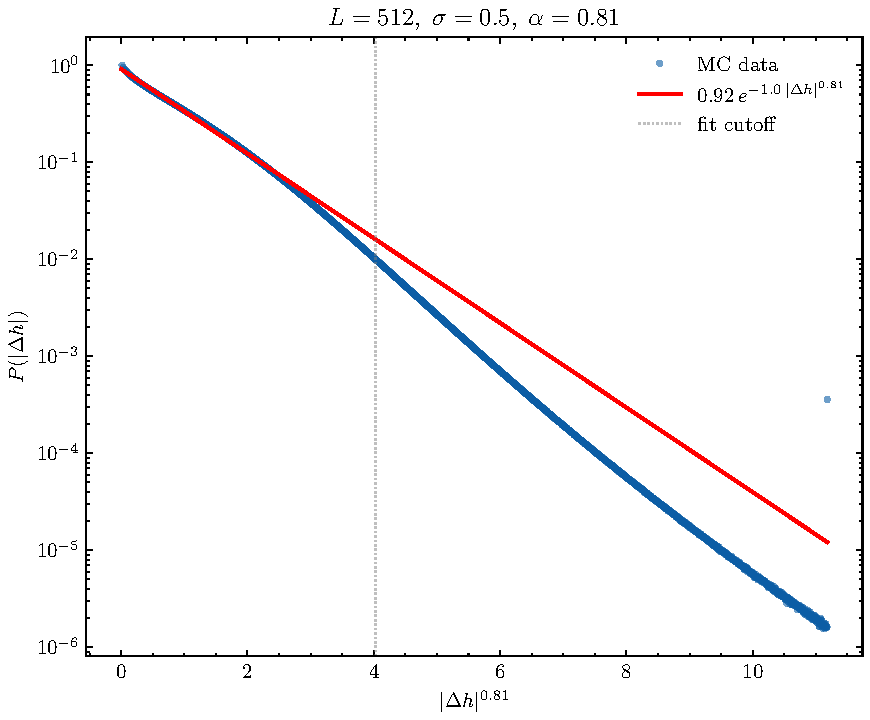
\includegraphics[width=0.44\textwidth]{../figures/histogram/hist_L512_s0.5.pdf}
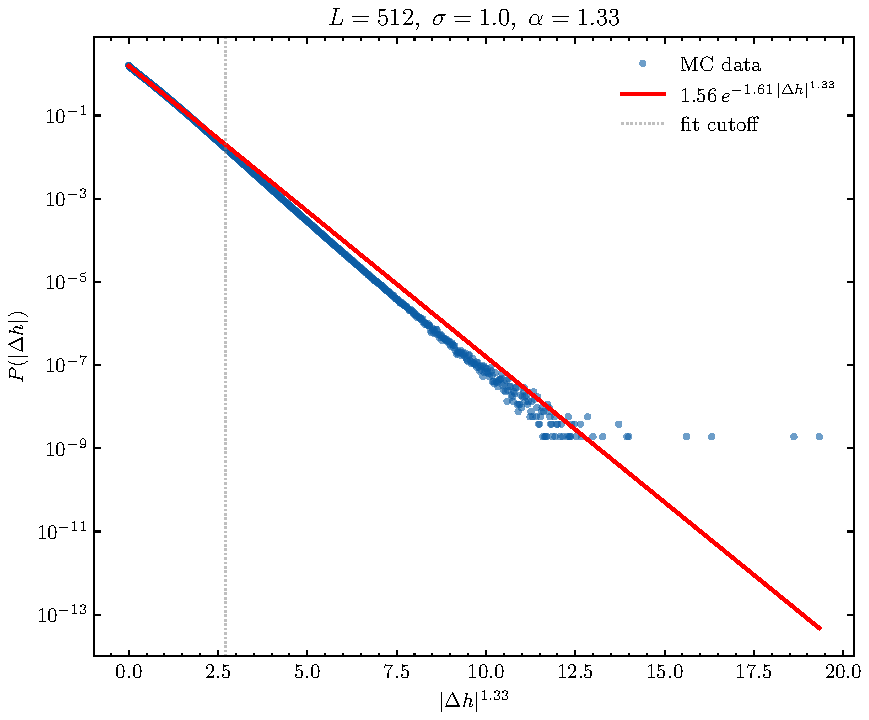
\includegraphics[width=0.44\textwidth]{../figures/histogram/hist_L512_s1.0.pdf}\\
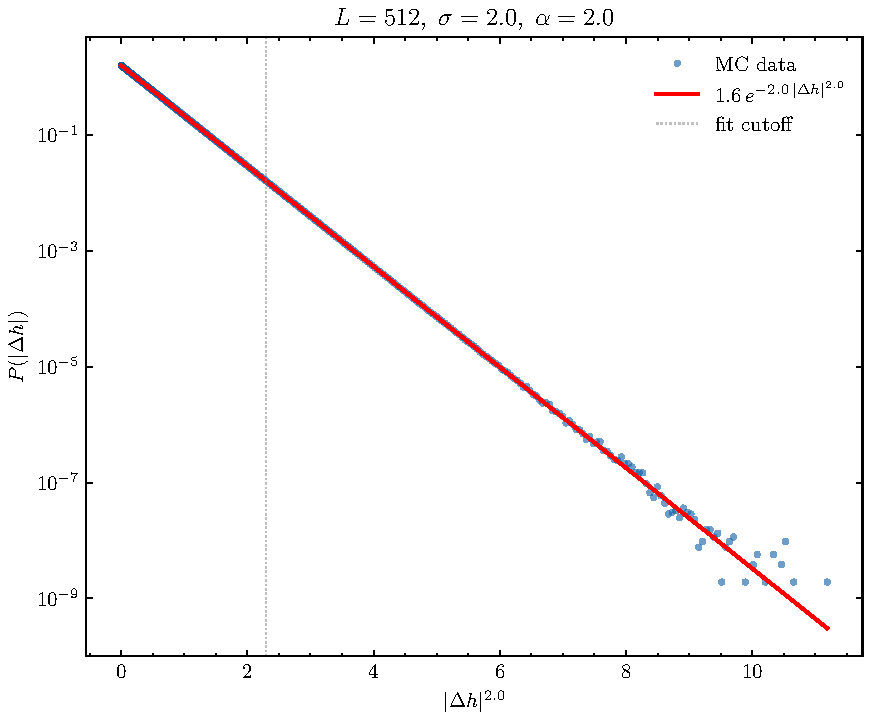
\includegraphics[width=0.44\textwidth]{../figures/histogram/hist_L512_s2.0.pdf}
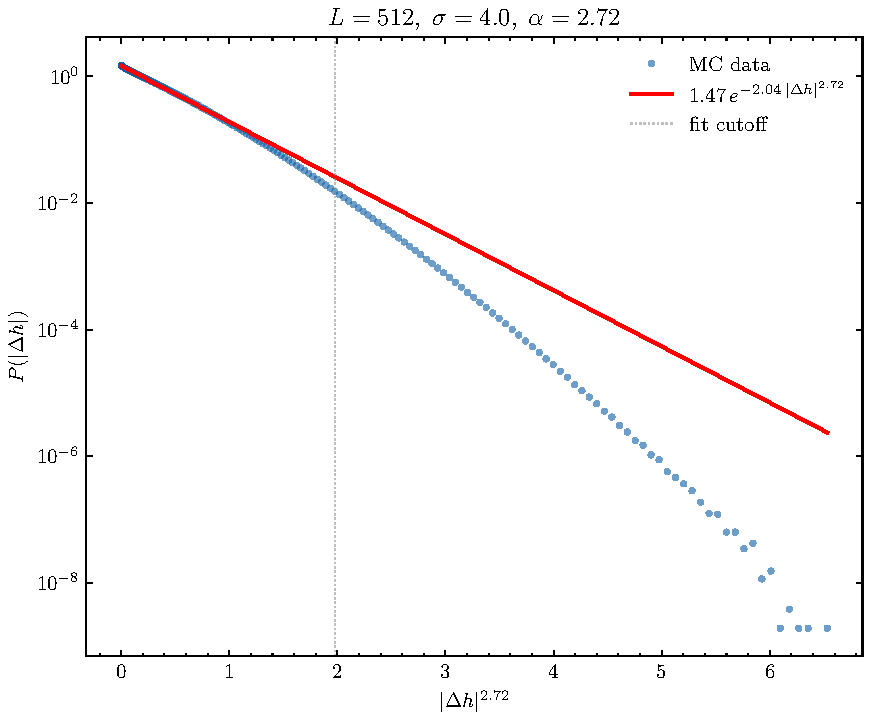
\includegraphics[width=0.44\textwidth]{../figures/histogram/hist_L512_s4.0.pdf}
\caption{Height difference distribution $P(|\Delta h|)$ for $L=512$ at
different $\sigma$, plotted in linearized coordinates ($\log P$ vs.\
$|\Delta h|^\alpha$) with free $\alpha$. The red line is the
stretched-exponential fit to the core region (left of the dotted line).
In these coordinates the fit is a straight line; deviations beyond the cutoff
reflect subleading corrections from the lattice.}
\label{fig:hist_fit}
\end{figure}

\FloatBarrier

%% ============================================================
\FloatBarrier
\subsection{Full Structure Factor}
%% ============================================================

The structure factor $S(k_x)=\langle|\hat{h}_{k_x}|^2\rangle$ is computed via
FFT along the $x$-direction only ($k_y=0$), avoiding the radial averaging
over both lattice directions that could mix anisotropic lattice artifacts.
The power law $S(k_x)=A/|k_x|^\gamma$ is fitted using only the small-$k$
regime ($|k_x|<0.5$) by log--log linear regression (OLS).

\begin{table}[htbp]
\centering
\caption{Power-law fit $S(k_x)=A/|k_x|^\gamma$ for $|k_x|<0.5$ ($k_y=0$ direction only).}
\label{tab:sf}
\small
\begin{tabular}{ccS[table-format=1.4(4)]S[table-format=1.4(4)]S[table-format=1.4]}
\toprule
$L$ & $\sigma$ & {$A$} & {$\gamma$} & {$R^2$} \\
\midrule
\multirow{4}{*}{64}
 & 0.5 & 6.0811(240) & 1.9755(32) & 0.9998 \\
 & 1.0 & 0.8723(33)  & 1.9890(31) & 0.9998 \\
 & 2.0 & 0.5147(20)  & 1.9851(32) & 0.9998 \\
 & 4.0 & 0.4578(21)  & 1.9916(37) & 0.9997 \\
\midrule
\multirow{4}{*}{256}
 & 0.5 & 6.0579(55) & 1.9833(7) & 0.9998 \\
 & 1.0 & 0.8689(8)  & 1.9905(7) & 0.9999 \\
 & 2.0 & 0.5094(4)  & 1.9907(7) & 0.9999 \\
 & 4.0 & 0.4560(4)  & 1.9946(7) & 0.9998 \\
\midrule
\multirow{4}{*}{512}
 & 0.5 & 6.0502(28) & 1.9824(4) & 0.9998 \\
 & 1.0 & 0.8684(4)  & 1.9906(3) & 0.9999 \\
 & 2.0 & 0.5087(2)  & 1.9920(3) & 0.9999 \\
 & 4.0 & 0.4571(2)  & 1.9918(3) & 0.9999 \\
\bottomrule
\end{tabular}
\end{table}

All exponents converge to $\gamma\approx 2$ with increasing $L$, confirming
the universal long-wavelength form $S(k)\propto 1/k^2$ for every $\sigma$
considered here. The non-universal dependence on $\sigma$ enters through the
amplitude: $A(\sigma=0.5)\approx 6.05$ whereas $A(\sigma=4.0)\approx 0.46$,
consistent with a softer interface at small $\sigma$ and a stiffer one at
large $\sigma$.

\begin{figure}[htbp]
\centering
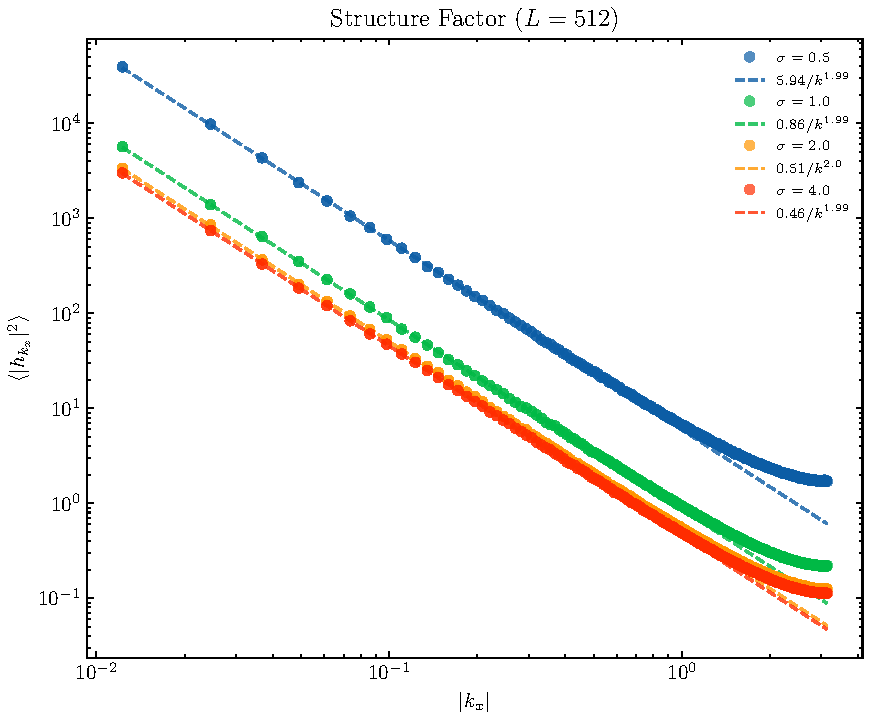
\includegraphics[width=0.75\textwidth]{../figures/structure_factor_full_L512.pdf}
\caption{Structure factor $S(k_x)=\langle|\hat{h}_{k_x}|^2\rangle$ vs.\ $|k_x|$
for $L=512$ at different $\sigma$ ($k_y=0$ direction only), with power-law
fits (dashed lines) from the small-$k$ regime.}
\label{fig:sf_L512}
\end{figure}

%% ============================================================
\FloatBarrier
\clearpage
\section{Coarse-Graining Analysis}
%% ============================================================

To probe the renormalization group (RG) flow of the generalized SOS model,
we perform a real-space coarse-graining (CG) analysis on an $L=1024$ system.
Starting from the original height field $h_i$, we iteratively apply $2\times 2$
block averaging:
\begin{equation}
  \bar{h}_I^{(b)} = \frac{1}{4}\sum_{i\in\text{block}\,I} h_i,
\end{equation}
producing coarse-grained fields at block sizes $b=1,2,4,\ldots,128$
on effective lattices of size $M=L/b$.
At each CG level we measure the nearest-neighbor height difference
distribution $P(|\Delta\bar{h}|)$, its moments, and the shell-averaged
structure factor.

\subsection{Excess Kurtosis: Approach to the Gaussian Fixed Point}

The excess kurtosis $\kappa_4 = \langle(\Delta h)^4\rangle/\langle(\Delta h)^2\rangle^2 - 3$
quantifies the non-Gaussianity of the height difference distribution.
For a Gaussian distribution, $\kappa_4=0$.

\begin{figure}[htbp]
\centering
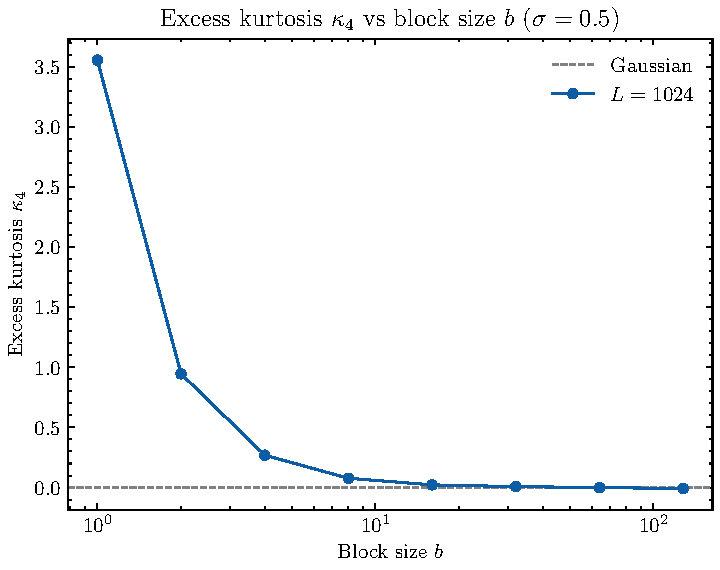
\includegraphics[width=0.48\textwidth]{../figures/coarse_grain/kurtosis_vs_b_s0.5.pdf}
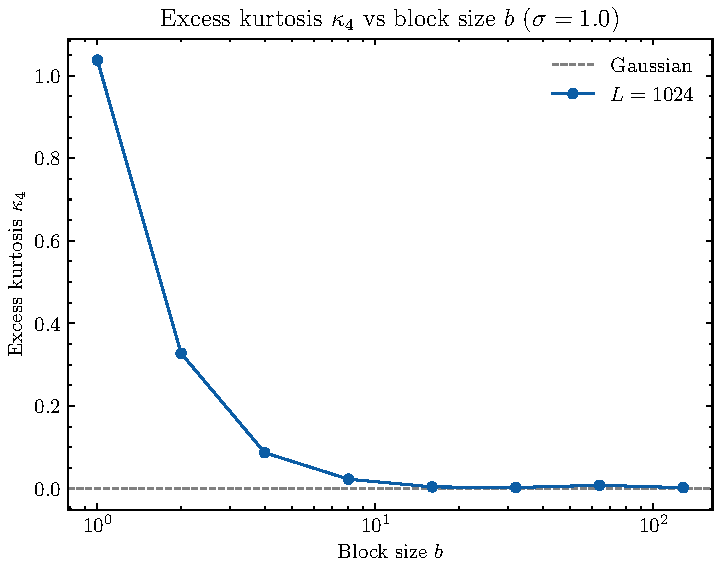
\includegraphics[width=0.48\textwidth]{../figures/coarse_grain/kurtosis_vs_b_s1.0.pdf}\\
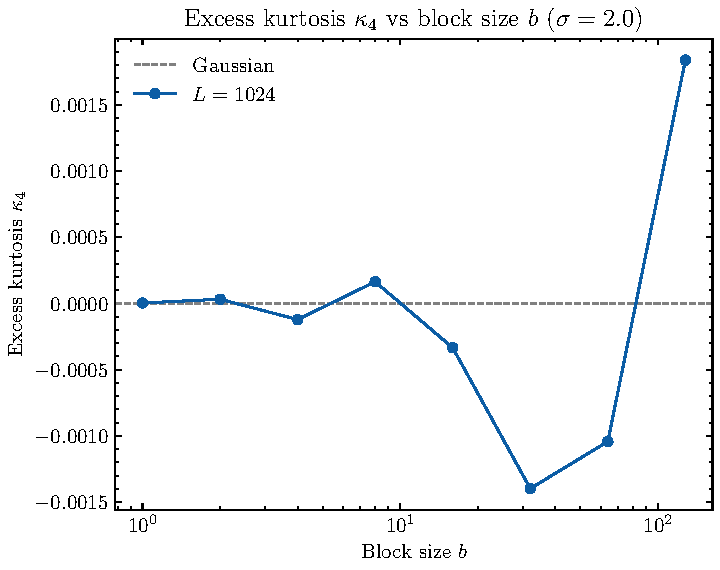
\includegraphics[width=0.48\textwidth]{../figures/coarse_grain/kurtosis_vs_b_s2.0.pdf}
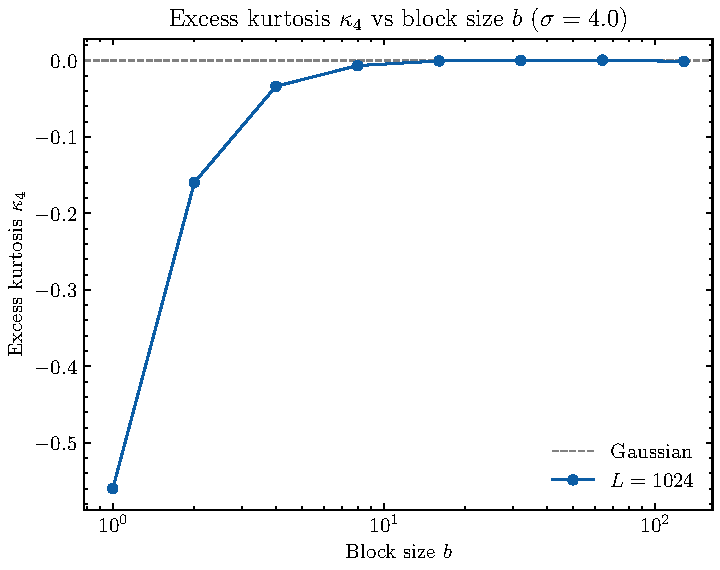
\includegraphics[width=0.48\textwidth]{../figures/coarse_grain/kurtosis_vs_b_s4.0.pdf}
\caption{Excess kurtosis $\kappa_4$ vs.\ block size $b$ for $L=1024$.
The dashed line marks the Gaussian value $\kappa_4=0$.
For all $\sigma$, the kurtosis flows rapidly toward zero under coarse-graining,
confirming the approach to the Gaussian fixed point.
The rate of convergence depends on $\sigma$: $\sigma=2.0$ is already Gaussian
at $b=1$, while $\sigma=0.5$ and $\sigma=4.0$ require $b\gtrsim 8$ to reach
$\kappa_4\approx 0$.}
\label{fig:kurtosis_vs_b}
\end{figure}

\FloatBarrier
\subsection{Height Difference Distribution under Coarse-Graining}

Figure~\ref{fig:hist_levels} shows the evolution of $P(|\Delta\bar{h}|)$
across CG levels, plotted against the rescaled variable
$|\Delta\bar{h}|^2/w^2$, where $w=\sqrt{\langle(\Delta\bar{h})^2\rangle}$
is the width at each CG level.
This rescaling collapses all Gaussian distributions onto a single universal
curve: in the Gaussian regime the half-normal law
\begin{equation}
  P(|\Delta\bar{h}|) =
  \sqrt{\frac{2}{\pi w^2}}
  \exp\!\left(-\frac{|\Delta\bar{h}|^2}{2w^2}\right)
\end{equation}
becomes a straight line when plotted as $\ln P$ vs.\ $|\Delta\bar{h}|^2/w^2$,
with universal slope $-1/2$ independent of $w$ (and hence of $\sigma$).

The actual onset of the Gaussian regime is determined from
Fig.~\ref{fig:kurtosis_vs_b}. Using the practical criterion
$|\kappa_4|<10^{-2}$, the first Gaussian-like block sizes are
$b_{\mathrm{G}}=32,16,1,8$ for $\sigma=0.5,1.0,2.0,4.0$, respectively.

As the coarse-graining level $b$ increases, the curves in each panel
progressively collapse onto the universal half-normal reference line (black
dashed). Deviations at small $b$ reflect the non-Gaussian character of the
bare interaction, which is washed out under the RG flow.
Table~\ref{tab:cg_halfnormal} lists the half-normal parameters at the common
Gaussian-regime scale $b=64$.

\begin{figure}[htbp]
\centering
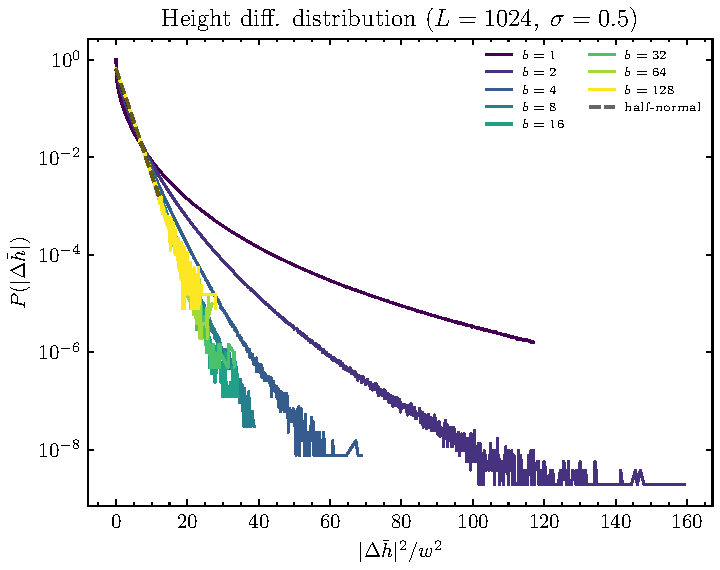
\includegraphics[width=0.44\textwidth]{../figures/coarse_grain/hist_levels_L1024_s0.5.pdf}
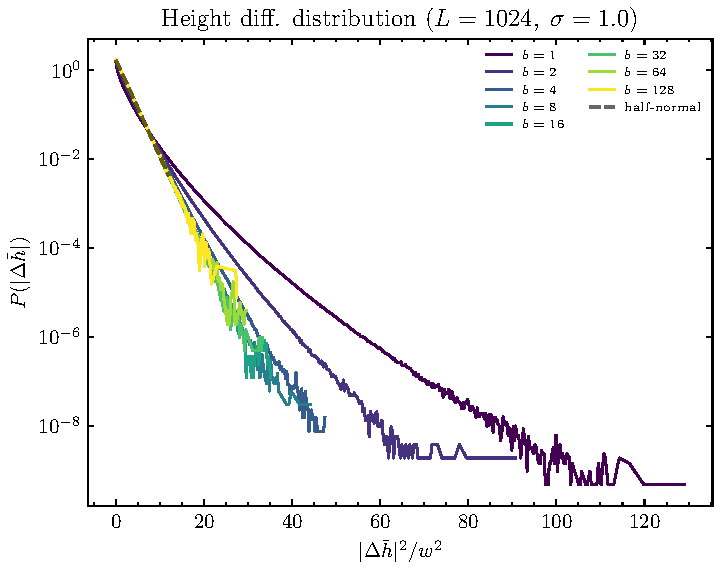
\includegraphics[width=0.44\textwidth]{../figures/coarse_grain/hist_levels_L1024_s1.0.pdf}\\
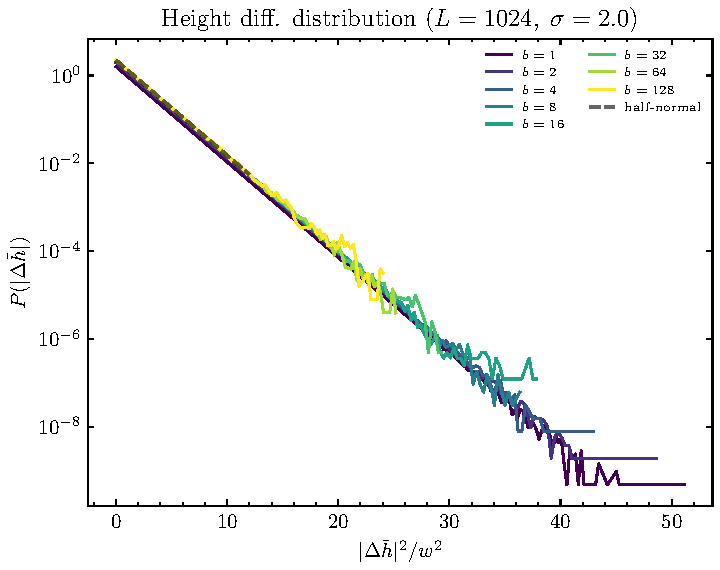
\includegraphics[width=0.44\textwidth]{../figures/coarse_grain/hist_levels_L1024_s2.0.pdf}
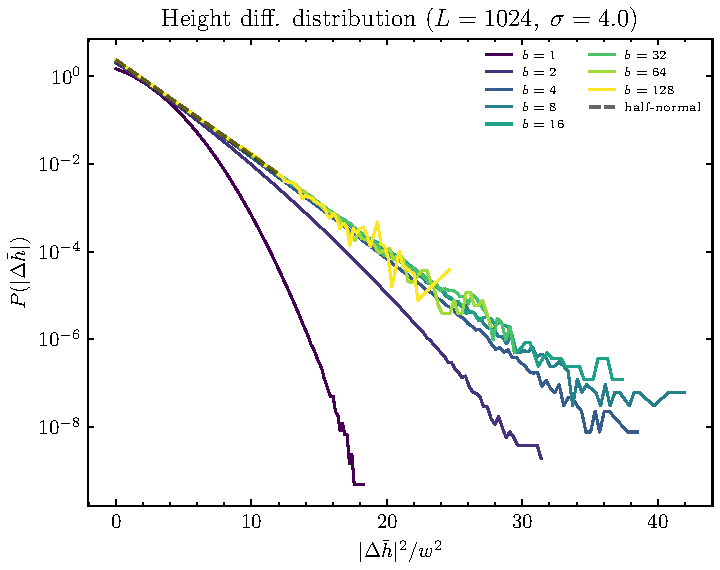
\includegraphics[width=0.44\textwidth]{../figures/coarse_grain/hist_levels_L1024_s4.0.pdf}
\caption{Height difference distribution $P(|\Delta\bar{h}|)$ at successive
CG levels ($b=1$ to $128$) for $L=1024$, plotted against the rescaled
variable $|\Delta\bar{h}|^2/w^2$. In the Gaussian regime, all curves
collapse onto the universal half-normal line (black dashed, slope $-1/2$
in log scale). Deviations at small $b$ reveal non-Gaussian local statistics
from the bare interaction.}
\label{fig:hist_levels}
\end{figure}

\begin{table}[htbp]
\centering
\caption{Half-normal parameters for $P(|\Delta\bar{h}|)$ at the common Gaussian-regime scale $b=64$ ($L=1024$). The amplitude is $A=\sqrt{2/\pi}/w$.}
\label{tab:cg_halfnormal}
\small
\begin{tabular}{c c S[table-format=+1.6] S[table-format=1.6] S[table-format=1.6]}
\toprule
$\sigma$ & {$b$} & {$\kappa_4$} & {$w$} & {$A$} \\
\midrule
0.5 & 64 & -0.000099 & 1.221002 & 0.653467 \\
1.0 & 64 &  0.008007 & 0.468195 & 1.704173 \\
2.0 & 64 & -0.001042 & 0.357661 & 2.230839 \\
4.0 & 64 &  0.000376 & 0.339290 & 2.351632 \\
\bottomrule
\end{tabular}
\end{table}

\FloatBarrier
\subsection{Structure Factor across CG Levels}

The shell-averaged structure factor $S(k) = \langle|\tilde{h}_k|^2\rangle$
is computed at each CG level.
Figure~\ref{fig:Sk_levels} shows that the $1/k^2$ power law is preserved
under coarse-graining for all four values of $\sigma$, as expected for a
system flowing to the Gaussian fixed point.
The amplitude decreases with $b$ because the block-averaged field has
smaller fluctuations.

\begin{figure}[!htbp]
\centering
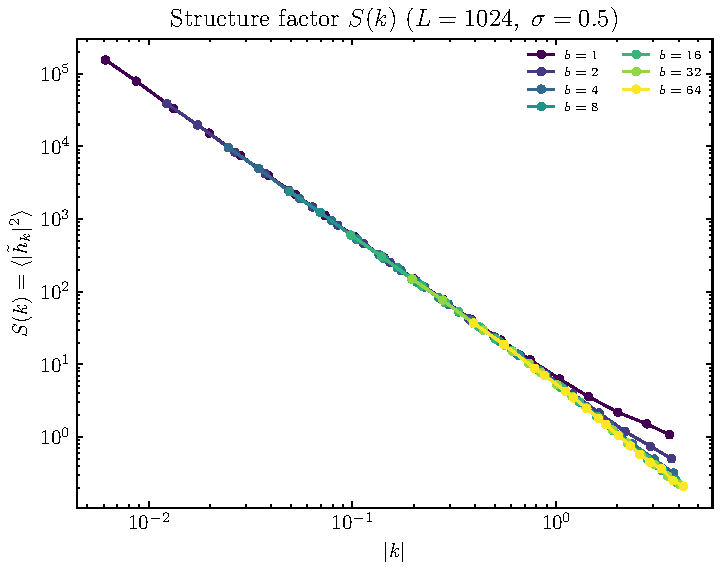
\includegraphics[width=0.39\textwidth]{../figures/coarse_grain/Sk_levels_L1024_s0.5.pdf}
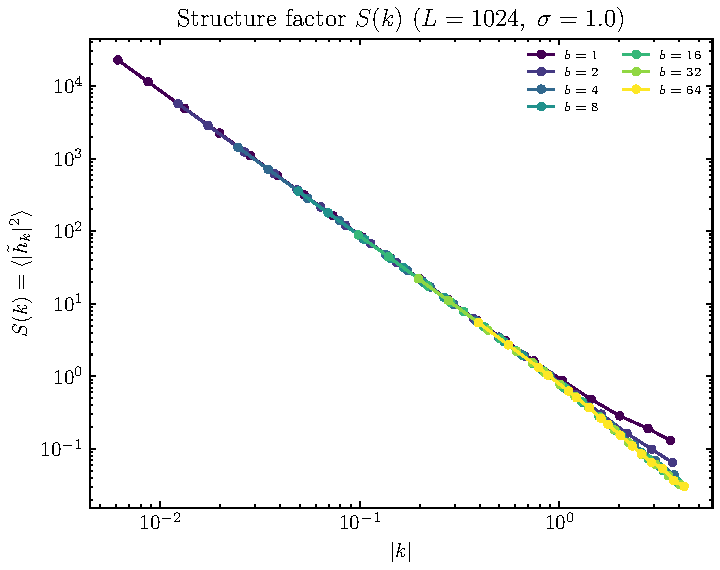
\includegraphics[width=0.39\textwidth]{../figures/coarse_grain/Sk_levels_L1024_s1.0.pdf}\\
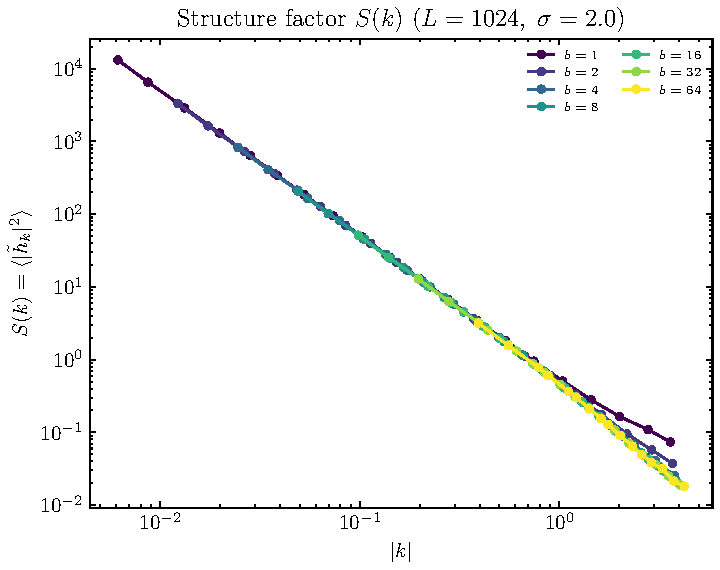
\includegraphics[width=0.39\textwidth]{../figures/coarse_grain/Sk_levels_L1024_s2.0.pdf}
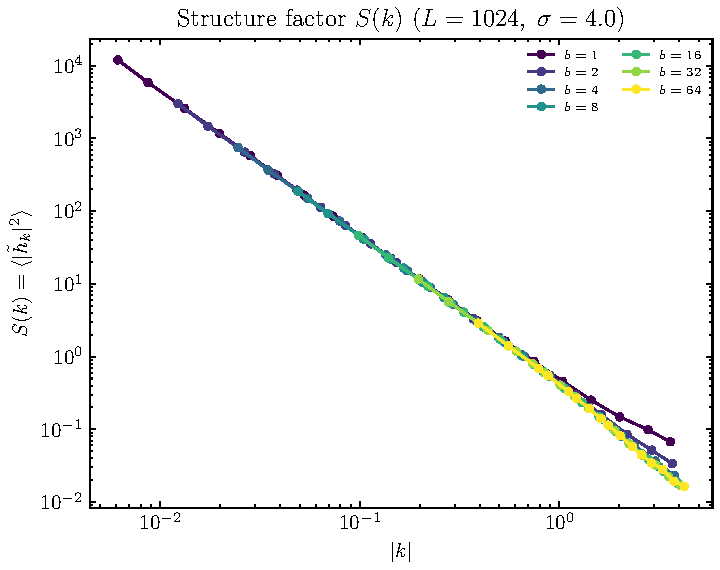
\includegraphics[width=0.39\textwidth]{../figures/coarse_grain/Sk_levels_L1024_s4.0.pdf}
\caption{Shell-averaged structure factor $S(k)$ at different CG levels
for $\sigma=0.5$, 1.0, 2.0, and 4.0, $L=1024$.
The $1/k^2$ scaling is maintained across all levels.}
\label{fig:Sk_levels}
\end{figure}

%% ============================================================
\FloatBarrier
\section{Discussion}
%% ============================================================

\subsection{Logarithmic Roughness and the Rough Phase}

For all values of $\sigma$ studied, the surface roughness $M^2$ grows
logarithmically with system size, $M^2 \sim a\ln L + b$.
This is the hallmark of a \emph{rough phase}, consistent with the
Mermin--Wagner theorem which forbids long-range order in two-dimensional
systems with continuous symmetry.

The prefactor $a$ depends strongly on $\sigma$: for $\sigma=0.5$,
$a\approx 0.93$, while for $\sigma=4.0$, $a\approx 0.071$.
Larger $\sigma$ penalizes height differences more steeply, leading to a
stiffer interface and smaller fluctuations.
The $\chi^2_\nu$ values show that including $L=4$ introduces noticeable
finite-size corrections (especially for $\sigma=0.5$), but the logarithmic
scaling becomes excellent for $L_{\min}\geq 8$.

\subsection{Structure Factor Scaling}

The structure factor $\chi_{k_{\min}}$ scales as $L^{\alpha}$ with
$\alpha \approx 2$ across all $\sigma$ values.
The physical reason is that, after coarse-graining, the long-wavelength sector
of the interface is described by the Gaussian elastic Hamiltonian
\begin{equation}
  \mathcal{H}_{\mathrm{eff}} \sim \frac{\gamma}{2}\sum_k k^2 |\hat{h}_k|^2,
\end{equation}
with an effective stiffness $\gamma$. Each Fourier mode therefore behaves like
an independent harmonic degree of freedom. By equipartition, each quadratic
mode carries an energy of order $T/2$, which implies
\begin{equation}
  \langle |\hat{h}_k|^2 \rangle \propto \frac{1}{k^2}
  \quad\Rightarrow\quad
  \chi_{k_{\min}} \propto L^2.
\end{equation}
Since the smallest nonzero wavevector scales as $k_{\min}=2\pi/L$, the
$1/k^2$ behavior directly gives $\chi_{k_{\min}}\sim L^2$.
The exponent $\alpha=2$ is universal and independent of $\sigma$, reflecting
the fact that the long-wavelength physics is governed by the Gaussian fixed
point regardless of the microscopic interaction exponent.

\subsection{Finite-Size Corrections}

The systematic fitting analysis reveals a clear pattern:
\begin{itemize}
\item At $L_{\min}=4$, the reduced $\chi^2_\nu$ is significantly larger
  than 1 for the structure factor fits (up to $\sim 50$ for $\sigma=4.0$),
  indicating strong finite-size corrections at the smallest sizes.
\item By $L_{\min}=8$ or 16, $\chi^2_\nu$ drops to $\mathcal{O}(1\text{--}3)$,
  and the fitted exponents converge to their asymptotic values.
\item The roughness fits are less sensitive to finite-size effects, with
  $\chi^2_\nu$ remaining moderate even when $L=4$ is included.
\end{itemize}

These observations suggest that $L\geq 8$ is sufficient for reliable
extraction of scaling exponents in this model, while $L=4$ should be
excluded from quantitative fits.

\subsection{Coarse-Graining and the Gaussian Fixed Point}

The coarse-graining analysis provides direct, real-space evidence for the
RG flow to the Gaussian fixed point.
Three independent diagnostics all point to the same conclusion:

\begin{enumerate}
\item The excess kurtosis $\kappa_4$ converges to zero within a few CG
  steps ($b\lesssim 8$) for all $\sigma$, indicating that the
  height difference distribution becomes Gaussian.

\item The histogram evolution provides a qualitative real-space picture
  consistent with this trend: as $b$ increases, the distribution narrows and
  its shape becomes progressively closer to Gaussian.

\item The structure factor maintains its $1/k^2$ scaling at all CG levels,
  consistent with a free-field (Gaussian) effective theory at long wavelengths.
\end{enumerate}

The special case $\sigma=2.0$ is already at the Gaussian fixed point
microscopically: the Boltzmann weight $e^{-K|\Delta h|^2}$ is Gaussian,
so $\kappa_4=0$ at every coarse-graining level.
For $\sigma\neq 2$, the bare interaction is non-Gaussian, but the
central limit theorem ensures that block-averaged variables become
Gaussian as the block size grows---precisely the mechanism underlying
the RG flow observed here.

\end{document}
